\documentclass[10pt,notes=hide]{beamer}
%Jonathan Dingel; PhD trade course

% PACKAGES
\usepackage{graphics}  % Support for images/figures
\usepackage{graphicx}  % Includes the \resizebox command
\usepackage{url}	   % Includes \urldef and \url commands
\usepackage{soul}      % Includes the underline \ul command
%\usepackage{framed}	   % Includes the \framed command for box around text
\usepackage{booktabs} %\toprule,\bottomrule
\usepackage{natbib}
\usepackage{bibentry}  % Includes the \nobibliography command
\usepackage{bbm}       %
%\usepackage{pgfpages}  %Supports "notes on second screen" option for beamer
\usepackage{verbatim}  %Supports comments
\usepackage{tikz}		%Supports graphing/drawing
\usepackage{pgfplots} %Supports graphing/drawing
\usepackage{amsfonts}  % Lots of stuff, including \mathbb 
\usepackage{amsmath}   % Standard math package
\usepackage{amsthm}    % Includes the comment functions
\usepackage{physics}

% CUSTOM DEFINITIONS
\urldef{\dingelhomepage}\url{faculty.chicagobooth.edu/jonathan.dingel/}
\urldef{\dingelemail}\url{jdingel@chicagobooth.edu}
\def\newblock{} %Get beamer to cooperate with BibTeX
\linespread{1.2}
\hypersetup{backref,pdfpagemode=FullScreen,colorlinks=true,linkcolor=blue,urlcolor=blue}
\newtheorem{proposition}{Proposition}
\newtheorem{assumption}{Assumption}

% IDENTIFYING INFORMATION
\title{International Macroeconomics and Trade}
\author{Jonathan I. Dingel}
\date{Autumn \the\year}

% BEAMER TEACHING STUFF
%\setbeameroption{show notes on second screen}
\setbeamertemplate{navigation symbols}{}  %Turn off navigation bar
%\setbeamertemplate{footline}{\begin{center}\textcolor{gray}{Dingel -- Managing the Firm in the Global Economy -- Week X -- \insertframenumber}\end{center}}

% THEMATIC OPTIONS
\definecolor{maroon}{RGB}{152,0,46}  %Booth maroon defined at http://staff.chicagobooth.edu/marketing/docs/email-signature-standards.pdf
\setbeamercovered{transparent=5}
\setbeamercolor{frametitle}{fg=maroon}
\setbeamercolor{item}{fg=maroon}
\usefonttheme{serif}

\setbeamertemplate{footline}{\begin{center}\textcolor{gray}{Dingel -- International Macroeconomics and Trade -- Week 7 -- \insertframenumber}\end{center}}
\begin{document}
% -----------------------------------------
%TITLE FRAME
\begin{frame}[plain]
\begin{center}
\large
\textcolor{maroon}{BUSN 33946 \& ECON 35101\\
International Macroeconomics and Trade\\ 
Jonathan Dingel\\
Autumn \the\year, Week 7}
\vfill 
\includegraphics[width=0.5\textwidth]{../images/chicago_booth_logo}
\end{center}
\end{frame}
% -----------------------------------------
\begin{frame}{Today: Heterogeneous firms}
\href{http://fordschool.umich.edu/rsie/workingpapers/Papers501-525/r509.pdf}{Hallak and Levinsohn}:
\begin{quote}
The problem with country-level data, in a nutshell, is that they are not sufficiently informative.
Countries do not produce anything and countries do not trade with one another.
Firms and consumers do these things.
Exactly how one intended or expected to measure the impact of trade on incomes without any reference to firms and/or households is something of a puzzle.
\end{quote}
\begin{itemize}
\item Brief introduction to firm-level facts
\item Work through Melitz (2003) model
\item Quick summaries of heterogeneous-firm papers
\end{itemize}
\end{frame}
% -----------------------------------------
\begin{frame}{Firms in international trade: Overview}
Five summary facts about firms in international trade
\begin{itemize}
\item Very few firms export:  4\% of 5.5 million US firms are exporters %BJRS JEP 2007
\item A few firms dominate exporting: top 10\% of exporters account for 96\% of exports  %BJRS JEP 2007
\item Exporters are bigger than non-exporters: Average exporting firm is twice the size of average non-exporter   %BJRS JEP 2007
\item Art Vandelay: More than 50\% of importing firms export  %Table 1 and maybe more from http://www.nber.org/chapters/c0500.pdf
\item Churning: About 10\% start or stop exporting annually %Dynamics
\end{itemize}
\end{frame}
% -----------------------------------------
\begin{frame}{Most manufacturing firms don't export}
%\begin{center}\includegraphics[width=.75\textwidth]{../images/BJRS_JEP_2007_tab2} \\ {\scriptsize \href{https://www.aeaweb.org/articles.php?doi=10.1257/jep.21.3.105}{Bernard, Jensen, Redding, Schott (\emph{JEP}, 2007)}}\end{center}
\begin{center}\includegraphics[height=.8\textheight]{../images/BernardJensenReddingSchott2018_tab1.pdf} \\ {\scriptsize \href{https://pubs.aeaweb.org/doi/pdf/10.1257/jel.20160792}{Bernard, Jensen, Redding, Schott (\emph{JEL}, 2018)}}\end{center}
\vspace{-1mm}
{\footnotesize We \href{https://tradediversion.net/2018/11/11/what-share-of-us-manufacturing-firms-export/}{used to think} exporting was rarer; data sources matter.\par}
\end{frame}
% -----------------------------------------
\begin{frame}{A few firms dominate exporting}
\begin{center}\includegraphics[width=.79\textwidth]{../images/BJRS_JEP_2007_tab4} \\ {\scriptsize \href{https://www.aeaweb.org/articles.php?doi=10.1257/jep.21.3.105}{Bernard, Jensen, Redding, Schott (\emph{JEP}, 2007)}}\end{center}
\end{frame}
% -----------------------------------------
\begin{frame}{Exporters are bigger than non-exporters}
\begin{center}\includegraphics[width=.95\textwidth]{../images/BJRS_JEP_2007_tab3}  \\ {\scriptsize \href{https://www.aeaweb.org/articles.php?doi=10.1257/jep.21.3.105}{Bernard, Jensen, Redding, Schott (\emph{JEP}, 2007)}} \end{center}
\end{frame}
% -----------------------------------------
\begin{frame}{Productivity premia}
\begin{center}\includegraphics[height=.85\textheight]{../images/BernardEatonJensenKortum2003_fig2b.pdf}  \\ {\scriptsize \href{}{Bernard, Eaton, Jensen, Kortum (\textit{AER}, 2003)}} \end{center}
\end{frame}
% -----------------------------------------
\begin{frame}{Importers, exporters, and multinationals}
\only<1>{\begin{center}\includegraphics[width=\textwidth]{../images/BJS_NBER_2009_tab1} \\ {\scriptsize \href{http://www.nber.org/chapters/c0500}{Bernard, Jensen, Schott (\emph{NBER}, 2009)}} \end{center}}
\end{frame}
% -----------------------------------------
\begin{frame}{Importers, exporters, and multinationals}
\only<1>{\begin{center}\includegraphics[width=\textwidth]{../images/BJS_NBER_2009_tab13} \\ {\scriptsize \href{http://www.nber.org/chapters/c0500}{Bernard, Jensen, Schott (\emph{NBER}, 2009)}} \end{center}}
\end{frame}
% -----------------------------------------
\begin{frame}{Exporting dynamics}
\begin{itemize}
  \item Considerable churning (\href{http://www.philadelphiafed.org/research-and-data/publications/business-review/2010/q4/brq410_understanding-exports-from-the-plant-up.pdf}{Alessandria and Choi 2010}): 
  \begin{center}\includegraphics[width=.7\textwidth]{../images/AlessandriaChoi2010}\end{center}
  \item Future exporters are larger and faster-growing than other non-exporters (\href{http://www.sciencedirect.com.proxy.uchicago.edu/science/article/pii/S0022199698000270}{Bernard and Jensen \emph{JIE} 1999})
  \item Exporters are more likely to enter new markets geographically contiguous with current export destinations (\href{http://www.martinalawless.com/Papers/marginaldistance.pdf}{Lawless \emph{OER} 2013})
  \item Sharing a border reduces estimated entry cost for Chilean chemical manufacturers by 20\%-40\% (\href{https://sites.google.com/site/edumoralescasado/files/ExtendedGravity.pdf?attredirects=0}{Morales et al 2015})
\end{itemize}
\end{frame}
% -----------------------------------------
\begin{frame}{More exporter premia}
Exporting firms\dots
\begin{itemize}
\item produce more products (BJRS 2007, BRS 2011)
\item pay higher wages (Frias, Kaplan, and Verhoogen 2009)
\item use more expensive material inputs (Kugler and Verhoogen 2012)
\item innovate more (Aw, Roberts and Xu 2011)
\end{itemize}
\end{frame}
% -----------------------------------------
\begin{frame}{Trade liberalization and reallocation across firms}
\begin{itemize}
\item Decompose change in aggregate productivity into between- and within-firm components
\item Finding that trade liberalization raised shares of more productive firms motived theoretical work on heterogeneous firms
\item Measuring firm-level TFP is plagued by simultaneity and selection biases
\item Measuring TFP is hard: see recent survey by Jan de Loecker and Penny Goldberg that emphasizes profitability vs productivity, TFPQ vs TFPR, markups, learning by exporting, and so forth
\item Pavcnik (2002) is an early and influential paper that applied Olley and Pakes (1996) technique to estimate TFP and assess Chile's 1970s trade liberalization
\end{itemize}
\end{frame}
% -----------------------------------------
\begin{frame}{Pavcnik (2002)}
\begin{itemize}
\item Chile liberalized trade 1974-1979 (tariffs ``often surpassing 100\% in 1974'' reduced to uniform 10\%)
\item Pavcnik has plant-level panel data for 1979-1986
\item No plant-level data on exporting behavior
\item Classify industries as import-competing, export-oriented, or non-tradable based on penetration (doesn't use tariff rates)
\item Exit is important: 35\% of plants exited between 1979 and 1986; exiting plants on average 8\% less productive than survivors
\item Industry productivity growth decomposed into unweighted average and share-productivity covariance (Table 3) shows 2/3 of aggregate productivity improvement due to between-plant shifts
\item Industry productivity regressed on orientation $\times$ year dummies (Table 4) shows substantial productivity increases 1979-1986 for import-competing sectors compared to non-tradables and no such improvements for export-oriented sectors
\end{itemize}
\end{frame}
% -----------------------------------------
\begin{frame}{Melitz (Ecma 2003)}
\begin{itemize}
\item Melitz (2003) is a model with heterogeneous firms and fixed costs of exporting that can speak to productivity premia and trade liberalization causing intra-industry reallocation
\item One of the most cited papers of last 20 years (\href{https://scholar.google.com/citations?user=SqlfKBsAAAAJ&hl=en&oi=ao}{12k GS})
\item Two building blocks:
\begin{enumerate}
	\item Krugman (AER 1980): CES preferences, IRS technology, monopolistic competition
	\item Hopenhayn (JPE 1992): equilibrium model of entry and exit
\end{enumerate}
\item Are trade-induced reallocations of labor from less to more productive firms a ``new'' source of gains from trade?
\end{itemize}
\end{frame}
% -----------------------------------------
\begin{frame}{Preferences and production}
As in Krugman (1980), representative agent has CES preferences:
$$ U = \left[\int_{\omega\in\Omega} q(\omega)^{\frac{\sigma-1}{\sigma}} \textrm{d} \omega \right]^{\frac{\sigma}{\sigma-1}} $$
Consumption and expenditure on each variety are
$$
q(\omega) = Q \left[\frac{p(\omega)}{P}\right]^{-\sigma}
\qquad
r(\omega) = R \left[\frac{p(\omega)}{P}\right]^{1-\sigma}
$$
where $P\equiv \left[\int_{\omega\in\Omega} p(\omega)^{1-\sigma} \textrm{d} \omega \right]^{\frac{1}{1-\sigma}}$
and $R\equiv \int_{\omega\in\Omega} r(\omega) \textrm{d} \omega$
\medskip
As in Krugman (1980), endowed labor $L$ is only factor of production with wage $w$ and IRS production function has fixed cost and constant marginal cost
\begin{align*}
l = f + q/\varphi 
&& 
p(\varphi) = \frac{\sigma}{\sigma-1}\frac{w}{\varphi}
\\
r(\varphi) = R \left(P\rho\varphi\right)^{\sigma-1} 
&&
\pi(\varphi) = \frac{1}{\sigma} r(\varphi) - f
\end{align*}
\end{frame}
% -----------------------------------------
\begin{frame}{Decentralized equilibrium is efficient}
See \href{https://www.jstor.org/stable/1831401}{Dixit and Stiglitz (1977)} and \href{https://www.journals.uchicago.edu/doi/pdfplus/10.1086/700732}{Dhingra and Morrow (2019)}
\begin{itemize}
\item Decentralized equilibrium solves:
$$
\max_{q_i,n} \int_{0}^{n} p_i(q_i) q_i \textrm{d}i 
\qquad
\text{ s.t. }
nf +  \int_{0}^{n} q_i / \varphi_{i} \textrm{d}i \leq L
$$
\item Social planner solves:
$$
\max_{q_i,n} \int_{0}^{n} q_i^{\frac{\sigma-1}{\sigma}} \textrm{d}i 
\qquad
\text{ s.t. }
nf +  \int_{0}^{n} q_i / \varphi_{i} \textrm{d}i \leq L
$$
\item CES preferences and constant marginal costs make 
$r(\varphi) \propto \varphi^{\sigma-1}, q(\varphi) \propto \varphi^{\sigma}\Rightarrow p_i(q_i) q_i \propto q_i^{\frac{\sigma-1}{\sigma}}$, so solutions coincide
\item Thus, many aggregate properties of Melitz (2003) coincide with those of perfectly competitive models
\item As is so often the case, CES is a very special demand system
\end{itemize}
\end{frame}
% -----------------------------------------
\begin{frame}{Aggregate outcomes (closed economy)}
\begin{itemize}
\item Since all firms with productivity $\varphi$ charge same price $p(\varphi)$,
$$
P
\equiv
\left[\int_{\omega\in\Omega} p(\omega)^{1-\sigma} \textrm{d} \omega \right]^{\frac{1}{1-\sigma}} 
=
\left[\int_{0}^{+\infty} p(\varphi)^{1-\sigma} M \mu(\varphi) \textrm{d} \varphi \right]^{\frac{1}{1-\sigma}} 
$$
where $M$ is mass of active firms and $\mu(\varphi)$ conditional pdf of active productivities in equilibrium
\item Using $p(\varphi) = \frac{\sigma}{\sigma-1}\frac{w}{\varphi}$, write this as $P = \frac{\sigma}{\sigma-1} w M^{\frac{1}{1-\sigma}} \tilde{\varphi}$
$$
\tilde{\varphi} \equiv \left[\int_{0}^{+\infty} \varphi^{\sigma-1} \mu(\varphi) \textrm{d} \varphi \right]^{\frac{1}{\sigma-1}}
$$
\item Similarly, other aggregate variables can be written
$$
R = M r(\tilde{\varphi})
\quad
\Pi = M \pi(\tilde{\varphi})
\quad
Q = M^{\frac{\sigma}{\sigma-1}} q(\tilde{\varphi})
$$
\item Aggregates are same as those in a Krugman model with mass $M$ of homogeneous firms with productivity $\tilde{\varphi}$
\item But $\tilde{\varphi}$ is endogenous and may depend on trade costs
\end{itemize}
\end{frame}
% -----------------------------------------
\begin{frame}{Entry and exit}
To determine equilibrium $\mu(\varphi)$ and $\tilde{\varphi}$, must specify the entry and exit process for firms. 
Similar to Hopenhayn (1992):
\begin{enumerate}
\item There is a large pool of identical potential entrants
\item Entrants pay a fixed cost of entry $f_e>0$ and draw productivity $\varphi$ from $G(\cdot)$
\item After observing their $\varphi$, firm chooses to produce or exit
\item Active firms exogenously exit with constant probability of death $\delta$
\end{enumerate}
\begin{itemize}
	\item In stationary equilibrium, active firm earns $\pi(\varphi)$ each period
	\item There is a unique productivity cutoff $\varphi^*$ and, given the fixed cost, it is defined by $\pi(\varphi^*)=0$
	\item The conditional pdf $\mu(\varphi) = \frac{g(\varphi)}{1-G(\varphi^*)}$ on support $[\varphi^*,\infty)$
\end{itemize}
\end{frame}
% -----------------------------------------
\begin{frame}{Free-entry and zero-cutoff conditions}
Free-entry condition
\begin{itemize}
\item Entry cost equals expected profits $f_e = \frac{1}{\delta} \frac{\Pi}{M} \left[1-G(\varphi^*)\right] $
\item Free-entry condition is therefore
$$ \bar{\pi} \equiv \frac{\Pi}{M} = \frac{\delta f_e}{1-G(\varphi^*)}$$
\item Higher cutoff $\Rightarrow$ entrants need higher average profits for survivors
\end{itemize}
Zero-cutoff condition
\begin{itemize}
	\item By definition of $\bar{\pi}$,
	$$ \bar{\pi} = \pi(\tilde{\varphi}(\varphi^*)) \iff 
	\bar{\pi} = 
	\pi(\varphi) = \frac{1}{\sigma} r(\tilde{\varphi}(\varphi^*)) - f
	$$
	\item By definition of $\varphi^*$,
	$ \pi(\varphi^*)=0 \iff r(\varphi^*) = \sigma f $
	\item Zero-cutoff condition is therefore
	$$ \bar{\pi} = f \left[\left(\frac{\tilde{\varphi}(\varphi^*)}{\varphi^*}\right)^{\sigma-1} - 1\right] $$
\end{itemize}
\end{frame}
% -----------------------------------------
\begin{frame}{Equilibrium $\varphi^*$ and $\bar{\pi}$}
\includegraphics[width=.9\textwidth]{../images/Melitz2003_fig1.pdf}
\begin{itemize}
\item Both free-entry and zero-cutoff conditions are independent of $L$
\item Zero-cutoff condition is not necessarily downward sloping
\item For Pareto distribution ($1 - G(\varphi) = a \varphi^b$), $\frac{\tilde{\varphi}(\varphi^*)}{\varphi^*}$ is constant so ZCP is horizontal
\end{itemize}
\end{frame}
% -----------------------------------------
\begin{frame}{Size, varieties, welfare, and free-trade equilibrium}
\begin{itemize}
\item Equilibrium still requires determination of $M$, obtain that from total labor hired, as in Krugman (1980)
\item Set wage as numeraire
\item Free entry and labor market clearing say $L=R = M r(\tilde{\varphi})$
$\Rightarrow M = \frac{1}{\sigma(\bar{\pi} + f)} L $
\item Welfare is $U = 1/P = \frac{\sigma-1}{\sigma} M^{\frac{1}{\sigma-1}} \tilde{\varphi}$
\item Since $\bar{\pi}$ and $\varphi^*$ are independent of size, 
greater size and costless trade are essentially isomorphic, as in Krugman (1980)
\item There is no reallocation of market shares across firms when comparing autarky and free trade
\end{itemize}
\end{frame}
% -----------------------------------------
\begin{frame}{Introducing trade costs}
\begin{itemize}
\item (Assume identical country sizes to shut down terms of trade)
\item Iceberg trade costs $\tau$ and fixed export cost $f_x$
\item Prices are
$p_d(\varphi) = \frac{\sigma}{\sigma-1} \frac{1}{\varphi}$
and
$p_x(\varphi) = \frac{\sigma}{\sigma-1} \frac{\tau}{\varphi}$
\item Revenues are
$$r_d(\varphi) = R_d \left(P_d\rho\varphi\right)^{\sigma-1}
\qquad
r_x(\varphi) = \tau^{1-\sigma}R_x \left(P_x\rho\varphi\right)^{\sigma-1}$$
\item By symmetry, $P_d = P_x = P$ and $R_d = R_x = R$
\item Profits are
$$
\pi_d(\varphi) = \frac{1}{\sigma} r_d(\varphi) - f
\quad 
\pi_x(\varphi) = \frac{1}{\sigma} r_x(\varphi) - f_x
$$
\item Total profits are $\pi(\varphi) = \pi_d(\varphi) + \max\{0,\pi_x(\varphi)\}$
\item Cutoffs are now defined as $\varphi^*$ and $\varphi^*_x$
\item Assume $\tau^{\sigma-1}f_x > f$ so that there are non-exporters ($\varphi^*_x>\varphi^*$)
\item Draw the $\pi_d(\varphi), \pi_x(\varphi)$ functions against $\varphi^{\sigma-1}$
\end{itemize}
\end{frame}
% -----------------------------------------
\begin{frame}{Aggregate outcomes for open economy}
\begin{itemize}
\item In the open economy, aggregate productivity is now given by
$$
\tilde{\varphi}_t = 
\left\{\frac{M}{M_t}\tilde{\varphi}^{\sigma-1} + n \frac{M_x}{M_t} (\tilde{\varphi}_x/\tau)^{\sigma-1} \right\}
$$
\item $M_t \equiv M + n M_x$ is total number of varieties
\item $\tilde{\varphi} \equiv \left[ \frac{1}{1-G(\varphi^*)} \int_{\varphi^*}^{+\infty} \varphi^{\sigma-1} g(\varphi) \textrm{d} \varphi \right]^{\frac{1}{\sigma-1}}$ is average of all firms
\item $\tilde{\varphi}_x \equiv \left[ \frac{1}{1-G(\varphi_x^*)} \int_{\varphi_x^*}^{+\infty} \varphi^{\sigma-1} g(\varphi) \textrm{d} \varphi \right]^{\frac{1}{\sigma-1}}$ is average of exporters
\item We can again write aggregate variables in terms of $\tilde{\varphi}_t$ but this relies heavily on symmetry (welfare depends on productivity of foreign exporters!)
$$
P = \frac{1}{\rho} M_t^{\frac{1}{1-\sigma}} \tilde{\varphi}_t
\quad 
R = M_t r(\tilde{\varphi}_t)
\quad
\Pi = M_t \pi(\tilde{\varphi}_t)
\quad
Q = M_t^{\frac{\sigma}{\sigma-1}} q(\tilde{\varphi}_t)
$$
\end{itemize}
\end{frame}
% -----------------------------------------
\begin{frame}{Free-entry and zero-cutoff conditions in open economy}
\begin{itemize}
\item Free-entry condition is same as before ($\delta f_e = \bar{\pi}[1-G(\varphi^*)]$), recognizing that $\bar{\pi} = \pi_d(\tilde{\varphi}) + n p_x  \pi_x(\tilde{\varphi}_x)$ where $p_x = \frac{1-G({\varphi}_x^*)}{1-G(\varphi^*)}$.
\item Zero-cutoff condition is now derived from $r_d(\varphi^*) = \sigma f$ and $r_x(\varphi^*_x) = \sigma f_x$, which jointly imply
$$ 
\frac{r_x(\varphi^*_x)}{r_d(\varphi^*)} = \frac{f_x}{f}
\iff
\varphi^*_x = \varphi^* \tau (f_x /f)^{1/(\sigma-1)}
$$
\item Rearranging $\bar{\pi}$ to be a function of $\varphi^*$ delivers
$$
\bar{\pi} 
=
f \left[\left(\frac{\tilde{\varphi}(\varphi^*)}{\varphi^*}\right)^{\sigma-1} - 1\right]
+
n p_x f_x \left[\left(\frac{\tilde{\varphi}_x(\varphi^*)}{\varphi_x^*(\varphi^*)}\right)^{\sigma-1} - 1\right]
$$
\item This ZCP has shifted up relative to closed-economy ZCP
\end{itemize}
\end{frame}
% -----------------------------------------
\begin{frame}{The consequences of trade}
\begin{center}
\includegraphics[width=.85\textwidth]{../images/MelitzRedding2014_fig1_3.pdf} \\
Melitz and Redding (Handbook 2014), Figure 1.3
\end{center}
Trade (increase in $n$, decrease in $\tau$ or $f_x$) raises the $\varphi^*$ cutoff, reallocates input shares to more productive firms, and produces welfare gains
\end{frame}
% -----------------------------------------
\begin{frame}{Measuring productivity in Melitz (2003) setting}
\begin{itemize}
\item With only one input, output quantity per worker is TFPQ
\begin{equation*}
\frac{\text{physical output}}{\text{variable workers}}
=
\frac{\sum_{j=1}^{N}\tau _{ij}x_{ij}\left(\varphi\right)}
{\sum_{j=1}^{N}l_{ij}^{v}\left(\varphi\right) }
=
\varphi
\end{equation*}
\item We often do not see physical output (particularly for differentiated goods).
What if we use TFPR?
\begin{equation*}
\frac{\text{value of output}}{\text{variable workers}}
=\frac{\sum_{j=1}^{N}p_{ij}\left(\varphi\right) x_{ij}\left(\varphi\right)}
	{\sum_{j=1}^{N}l_{ij}^{v}\left(\varphi\right)}
=\frac{\sigma}{\sigma-1} w_{i}
\end{equation*}
\item Relative revenues and relative productivities:
\begin{equation*}
\frac{r(\varphi_1)}{r(\varphi_2)} = \left(\frac{\varphi_1}{\varphi_2}\right)^{\sigma-1}
\end{equation*}
\item Relate this to the productivity-quality isomorphism mentioned in footnote 7 of Melitz (2003)
\end{itemize}
\end{frame}
% -----------------------------------------
\begin{frame}{Bernard, Eaton, Jensen, and Kortum (2003)}
\begin{itemize}
\item BEJK (2003) introduce firm heterogeneity into a framework close to Eaton and Kortum (2002), analogous to what Melitz (2003) does for Krugman (1980)
\item Many countries, many industries, CES preferences
\item Many firms within each industry with CRS technologies, iceberg trade costs, and heterogeneous productivities competing on price
\item Price charged by least-cost firm in each industry is bounded by the second lowest cost (from same or different country)
\item The joint distribution of highest and second-highest productivities is key:
\begin{equation*}
F_j(z_1,z_2)
=
\Pr\left[Z_{1i}\leq z_1, Z_{2i}\leq z_2 \right]
=
\left[1+T_i\left(z_2^{-\theta} - z_1^{-\theta}\right)\right]\exp\left(-T_iz_2^{-\theta}\right)
\end{equation*}
\item Markup $M_n(j) = P_n(j)/C_{1n}(j)$ is random variable $M_n$ drawn from truncated Pareto (truncated by monopolist's markup)
\begin{equation*}
	H_n(M) = \Pr[M_n <m] = 1 -m^{-\theta} \quad 1 \leq m < \frac{\sigma}{\sigma-1}
\end{equation*}
\end{itemize}
\end{frame}
% -----------------------------------------
\begin{frame}{Revisiting many questions with firm heterogeneity }
\begin{itemize}
\item Multiple factors of production (Bernard Redding Schott 2007)
\item Variable markups (Melitz and Ottaviano 2008)
\item Trade elasticity (Chaney 2008)
\item Gravity regressions (Helpman Melitz Rubinstein 2008)
\item Multi-product firms (Benard Redding Schott 2009)
\item Structure of trade costs (Arkolakis 2010, Eaton Kortum Kramarz 2011)
\item Export vs FDI (Helpman Melitz Yeaple 2004)
\end{itemize}
See Melitz and Redding (2014) Handbook of International Economics chapter for overview of extensions
\end{frame}
% -----------------------------------------
\begin{frame}{Bernard, Redding, Schott (2007)}
\begin{itemize}
	\item Introduce multiple industries that vary in factor intensity and countries that vary in factor abundance
	\item Total cost function for firm in $i$ in industry $j$ using skilled $S$ and unskilled $U$ is
	$$
	\left[f_{ij}+q_{ij}/\varphi\right] w_{Si}^{\beta_j} w_{Ui}^{1-\beta_j}
	$$
	\item If $\tau=1$ and $f_x=0$, you're in FPE set and four theorems apply straightforwardly
	\item Absent FPE, trade affects intra-industry reallocation
	\item Growth of exporters is greater in comparative-advantage sector,
	so exit by less productive firms is stronger in the comparative-advantage sector
	\item Race between Stolper-Samuelson force and changes in product variety and average productivity
\end{itemize}
\end{frame}
% -----------------------------------------
\begin{frame}{Melitz and Ottaviano (2008)}
\begin{itemize}
	\item Firm heterogeneity a la Melitz (2003) with quasi-linear quadratic preferences 
	(due to Ottaviano, Tabuchi and Thisse 2002)
	\begin{equation*}
		U = 
		q_0^c 
		+ \int_{i\in \Omega} q_i^c \textrm{d}i 
		- \frac{1}{2} \gamma \int_{i\in \Omega} \left(q_i^c\right)^2 \textrm{d}i 
		- \frac{1}{2} \eta \left(\int_{i\in \Omega} q_i^c \textrm{d}i\right)^2
	\end{equation*}
	\item Linear demand delivers variable markups
	\item Market size affects markups, profits, and productivity cutoff in closed economy
	\item Asymmetric countries and trade costs analyzed thanks to freely traded outside good that equalizes wages
	\item Economic mechanisms not new (see Krugman 1979, Venables 1987), but integration of asymmetric countries, variable markups, and heterogeneous firms is novel
\end{itemize}
\end{frame}
% -----------------------------------------
\begin{frame}{Chaney (2008)}
\begin{itemize}
{\small
	\item In Krugman (1980, section II), exports from Home to Foreign are
	$$
	\frac{n \tau^{1-\sigma}}{n \tau^{1-\sigma} + n^*} w^*L^*
	=
	\frac{n}{n+n^* \tau^{\sigma-1}} w^*L^*
	$$
	\item Chaney extends Melitz (2003) to allow asymmetric countries and trade costs by introducing freely traded homogeneous good, fixed set of potential entrants, and a global mutual fund
	\item Pareto distribution for $\varphi$ delivers closed-form expressions
	\item The resulting gravity equation in sector $h$ is
	$$
	X_{ij}^{h}= \mu_h \frac{Y_i Y_j}{Y}
	\left(\frac{w_i \tau_{ij}^h}{\theta_j^h}\right)^{-\gamma_h}
	\left(f_{ij}^{h}\right)^{[(\sigma_h-1-\gamma_h)/(\sigma_h-1)]}
	$$
	where $\theta_j^h$ is a multilateral-resistance term and $\gamma_h$ is Pareto shape 
	\item In Krugman (1980), variable trade costs show up in intensive margin of revenues per firm
	\item In Chaney (2008), both variable and fixed trade costs affect revenues per firm and total number of exporting firms
	\item With Pareto, variable trade costs do not change average revenue per firm; only extensive margin matters, which depends on $\gamma$, not $\sigma$
}
\end{itemize}
\end{frame}
% -----------------------------------------
\begin{frame}{Helpman, Melitz, Rubinstein (2008)}
\begin{columns}
\begin{column}{.4\textwidth}
In Krugman, Melitz, and Chaney, bilateral (country-level) exports are always strictly positive. But zeros are pervasive.
HMR (2008) do Melitz with truncated Pareto productivity distributions 
\end{column}
\begin{column}{.6\textwidth}
\includegraphics[width=\textwidth]{../images/HelpmanMelitzRubinstein2008_fig1.pdf}
\end{column}
\end{columns}
\begin{itemize}
	\item Elasticity of \textit{firm}'s revenue wrt distance suffers OVB: 
	Greater trade cost also reduces number of exporting firms
	\item Elasticity also suffers selection bias: 
	Non-zero trade flows have lower unobserved trade costs for more distance partners
	\item Two-step estimation procedure to addresses these biases and exploit both trading and nontrading country pairs (not PPML; Heckman (1979) selection using entry costs or common religion)
\end{itemize}
\end{frame}
% -----------------------------------------
\begin{frame}{Bernard, Redding, Schott (2009)}
\begin{itemize}
	\item Recall 12\% of US exporters that sell 5+ products to 5+ destinations account for 92\% of export value
	\item BRS (2009) essentially do two-dimensional Melitz
	\item Nested CES preferences: CES over products and a continuum of firms supply differentiated varieties within each product
	\item Each firm draws two stochastic shocks: productivity common to all products and product-specific ``product attributes''
	\item Fixed cost of selling to each market and another product-market fixed cost
	\item Selection both within and across firms: Within exporters, products with the worst attributes are supplied only to the domestic market, while products with the best attributes are exported to the largest number of markets.
	\item Trade liberalization causes firms to drop their worst products
\end{itemize}
\end{frame}
% -----------------------------------------
\begin{frame}{Arkolakis (2010)}
Melitz's fixed-cost story faces an empirical tension
\begin{itemize}
	\item Only a small number of firms export, which suggests that fixed exporting costs are large
	\item Many exporters only export small amounts, which suggests that fixed exporting costs are small
	\item Arkolakis (2010) extends Chaney (2008) with endogenous marketing costs to explain size distribution of exporters
	\item Fixed cost of reaching consumers in $j$ with probability $x$ is
	$$
	f_{ij}(x) = f_{ij} \times \left[\frac{1-(1-x)^{1-\mu}}{1-\mu}\right]
	$$
	\item Same macro implications are Chaney (2008): Elasticity of aggregate trade flows wrt $\tau_{ij}$ is Pareto shape parameter
\end{itemize}
\end{frame}
% -----------------------------------------
\begin{frame}{Eaton, Kortum, Kramarz (2011)}
Quantitative exercise to move past Melitz's qualitative match. Motivating facts:
\begin{enumerate}
	\item Firms do not enter markets according to an exact hierarchy. 
	\item Their sales where they do enter deviate from the exact correlations the basic model insists on.
	\item Firms that export sell too much in France. 
	\item In the typical destination, there are too many firms selling small amounts.
\end{enumerate}
Approach:
\begin{itemize}
	\item Introduce market and firm-specific heterogeneity in entry costs and demand
	\item Incorporate Arkolakis (2010) formulation of market access costs
	\item Estimate via SMM: Raw efficiency (Melitz story) explains 57\% of variation in extensive margin
	\item Do a counterfactual cut in trade costs
\end{itemize}
\end{frame}
% -----------------------------------------
\begin{frame}{Helpman, Melitz, Yeaple (2004): Export vs FDI}
{\small A firm with productivity $\varphi$ facing domestic market $d$ and export market $x$ with demands $D_{\ell}(q_\ell) = B_\ell q_\ell^{\rho-1}$
may choose to export at fixed cost $f_x$ and marginal cost $m/\varphi + m_x$ or it may instead invest at fixed cost $f_i$ and marginal cost $m/\varphi$ (oversimplify with same MC for domestic and FDI):} 
\begin{align*}
\pi(\varphi) &= \pi_d(\varphi) + \max\{0,\pi_x(\varphi),\pi_i(\varphi) \} 
&
\pi_d (\varphi) &= B_d \left(1-\rho\right) \varphi^{\rho/(1-\rho)}
\\
\pi_x (\varphi) &= B_x \left(1-\rho\right) \left(\frac{\varphi}{1+\varphi m_x}\right)^{\rho/(1-\rho)} - f_x
\\
\pi_i (\varphi) &= B_x \left(1-\rho\right) \varphi^{\rho/(1-\rho)} - f_i
\end{align*}
To decide between exporting and investing, compare $\pi_x$ and $\pi_i$
\end{frame}
% -----------------------------------------
\begin{frame}{Proximity-concentration tradeoff}
\begin{itemize}
  \item If $f_i\leq f_x$, horizontal FDI is cheaper than exporting in both fixed costs ($f_i \leq f_x$) and marginal costs ($m < m + m_x$)
  \item If $f_i > f_x$, there is a proximity-concentration tradeoff because FDI involves \emph{higher} fixed cost and \emph{lower} marginal cost
\end{itemize}
To illustrate, let $\rho = \frac{1}{2}$ and $B_d = B_x$
\begin{center}
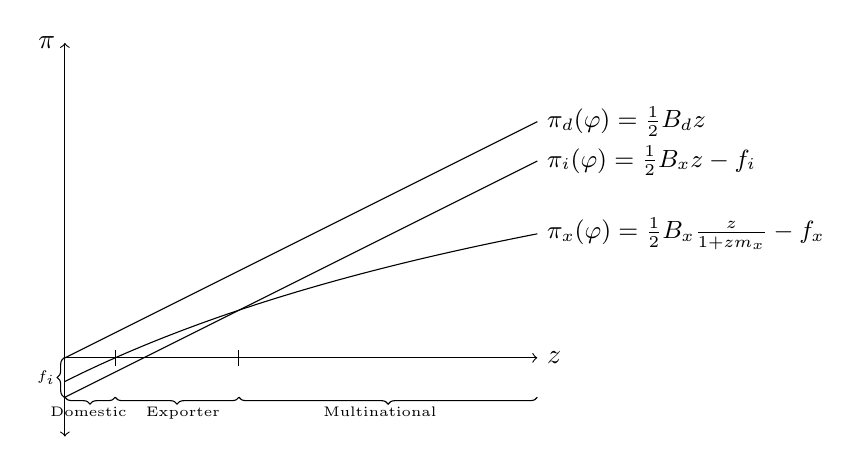
\begin{tikzpicture}[domain=0:6]
  \draw[->] (0,0) -- (6,0) node[right] {$z$};
  \draw[<->] (0,-1) -- (0,4) node[left] {$\pi$};
  \draw[domain=0:6,smooth,variable=\z,black] plot ({\z},{.5*\z});
  \draw[] (6,3) node[right] {\textcolor{black}{\small $\pi_d(\varphi) = \frac{1}{2} B_d z $}};
  \draw[domain=0:6,smooth,variable=\z,black] plot ({\z},{.5*(\z/(1+.1*\z)) - .3});
  \draw[] (6,1.575) node[right] {\textcolor{black}{\small $\pi_x(\varphi) = \frac{1}{2} B_x \frac{z}{1+z m_x} - f_x$}};
  \draw[domain=0:6,smooth,variable=\z,black] plot ({\z},{.5*\z -0.5});
  \draw[] (6,2.5) node[right] {\textcolor{black}{\small $\pi_i(\varphi) =  \frac{1}{2} B_x  z - f_i$}};
  \draw[decoration={brace,mirror},decorate] (-.01,0) -- (-.01,-.5); \draw[] (0,-.25) node[left] {\tiny $f_i$};
  %Show the partition:
  \draw[-] (0.6383,.1) -- (0.6383,-.1) ; 
\draw[-] (2.21,.1) -- (2.21,-.1) ;
  \draw[decoration={brace,mirror},decorate] (0,-.5) -- (0.6383,-.5); \draw[] (.3,-.5) node[below] {\tiny Domestic};
  \draw[decoration={brace,mirror},decorate] (0.6383,-.5) -- (2.21,-.5); \draw[] (1.5,-.5) node[below] {\tiny Exporter};
  \draw[decoration={brace,mirror},decorate] (2.21,-.5) -- (6,-.5); \draw[] (4,-.5) node[below] {\tiny Multinational};
\end{tikzpicture}
\end{center}
\end{frame}
% -----------------------------------------
\begin{frame}{Comparative statics}
\hypertarget{exportvsfdi}{}
For a firm comparing exporting and investing:
{
\begin{itemize}
  \item Higher productivity (higher $z$) makes investment relatively more attractive
  \item Higher trade costs (higher $m_x$ or $f_x$) make investment relatively more attractive %\hyperlink{app:exportvsfdi:compstat1}{\beamergotobutton{}}
  \item Higher plant fixed costs (higher $f_i$) make investment less attractive %\hyperlink{app:exportvsfdi:compstat2}{\beamergotobutton{}}
  \item Higher demand (higher $B_x$) makes investment more attractive %\hyperlink{app:exportvsfdi:compstat3}{\beamergotobutton{}}
\end{itemize}
}
\end{frame}
% -----------------------------------------
\begin{frame}{Trade and firm-level innovation}
{\small So far, firm's productivity $\varphi$ is a (randomly drawn) fixed characteristic}
\begin{itemize}
{\small 
\item Melitz and Trefler (JEP 2012) discuss gains from variety, reallocation of resources, and trade-induced innovation
\item Trade has a market-size effect on R\&D decisions (Schmookler 1954) [same logic as proximity-concentration tradeoff]
\item \href{https://academic.oup.com/qje/article-abstract/123/2/489/1930844}{Verhoogen (\textit{QJE}, 2008)} finds that '94 peso devaluation increased Mexican plants' exports and ISO-9000 certification
\item \href{http://qje.oxfordjournals.org.proxy.uchicago.edu/content/125/3/1051.short}{Lileeva and Trefler (\textit{QJE} 2010)}: Canadian firms that experienced larger tariff cuts under the US-Canadian FTA had greater labor productivity increases, engaged in more production innovation, and had higher adoption rates for advanced manufacturing technologies.
\item \href{https://academic.oup.com/qje/article/132/2/551/3002609}{Atkin, Khandelwal, Osman (\textit{QJE} 2017)}: Treated firms produce (fewer) higher-quality rugs. They have higher quality after controlling for specifications; perform better when asked to produce identical rugs; exhibit learning curves; and improve quality most along dimensions in which buyers and intermediary shared info.
}
\end{itemize}
\end{frame}
% -----------------------------------------
\begin{frame}{Atkeson and Burstein (2010)}
The argument
\begin{itemize}
\item Changes in trade costs can have large effects on individual firms' innovation decisions without affecting aggregate welfare
\end{itemize}
The model
\begin{itemize}
	\item Heterogeneous firms produce differentiated CES products incurring fixed and variable export costs as in Melitz (2003)
	\item Model of innovation builds on Griliches (1979)
	\item Firms profit opportunities determined by firm-specific factor (productivity)
	\item \textit{Process} innovation: Increase stock of specific factor in existing firm
	\item \textit{Product} innovation: Create new firms with new initial stock of factor
\end{itemize}
\end{frame}
% -----------------------------------------
\begin{frame}{Atkeson and Burstein (2010)}
What is the effect of a change in marginal trade costs on aggregate productivity?
\begin{itemize}
\item \textit{Direct effect} is change in aggregate productivity holding fixed firms' exit, export, process, and product innovation decisions
\item \textit{Indirect effect} is changes in firms' exit, export, process, and product innovation decisions caused by the change in trade costs
\item Krugman (1980) has only the product innovation margin
\item Main result: Adding firm heterogeneity and process innovation changes consequences for aggregate productivity little because 
the increase in productivity of average firm 
from changes in exit and export decisions and reallocation of process innovation from non-exporters to exporters 
is offset by production innovation
\item The logic: Firms' free-entry condition constrains the overall response of aggregate productivity to changes in trade costs
\item Lower trade costs raise innovation by current and prospective exporters, but this also reduces entrants' expected profits
\end{itemize}
\end{frame}
% -----------------------------------------
\begin{frame}{Atkeson and Burstein (2010)}
Innovation requires employing the research good
\begin{itemize}
	\item Process innovation: Invest $\exp(z)c(q)$ units to have 
	$\exp(z+\Delta_z)^{1/(\rho-1)}$ with probability $q$
	and
	$\exp(z-\Delta_z)^{1/(\rho-1)}$ with probability $1-q$
	with $c',c''>0$
	\item Product innovation: Invest $n_e$ units to produce new firm in $t+1$ with state variable $s$ drawn from $G$
\end{itemize}
Special case 1: All firms export ($n_x=0$)
\begin{itemize}
\item Absent fixed costs of exporting, a decline in the marginal cost of exporting affects all (active) firms' profits proportionally.
\item Free-entry condition requires this increase in profits be exactly offset by increase in cost of research good that produces both innovations.
\item The indirect effect corresponds entirely to a change in product innovation.
\end{itemize}
See paper for calibration and numerical results for $n_x>0$ case
\end{frame}
% -----------------------------------------
\begin{frame}{Coming up next}
In the next three weeks, we will turn to economic geography, including intranational trade
\begin{itemize}
\item Week 8: We introduce local increasing returns (agglomeration)
\item Week 9: We introduce models in which  monopolistic competition, trade costs, and mobile labor drive agglomeration
\item Week 10: Economic geography with heterogeneous skills
\end{itemize}
\end{frame}
% -----------------------------------------
\end{document}
